\section{Необходимый материал}
\subsection{Обозначения и основные определения}
\textbf{Конечные поля.} Существует, с точностью до изоморфизмов, единственное конечное поле, состоящее из \(2^n\) элементов, которое обозначается \(\text{GF}(2^n)\). В данной работе будет использоваться ''\(\oplus\)'' для обозначения сложения в поле, а \(a \odot b\) или \(ab\) для обозначения произведения \(a, b \in \text{GF}(2^n)\). Для всех \(x \in \text{GF}(2^n)\) выполняется \(x^{2^n} \oplus x = 0\).

Пусть \(n = 2m\), тогда определим отображение из \(\text{GF}(2^{2m})\) в \(\text{GF}(2^m)\) как функцию \(\text{Tr}_m: \text{GF}(2^{2m}) \rightarrow \text{GF}(2^m)\), такую, что \(\text{Tr}_m(x) = x^{2^m} \oplus x\). Для любого \(\beta \in \text{GF}(2^{2m})\), такого, что \(\text{Tr}_m(\beta) = 1\), элементы из \(\text{GF}(2^{2m})\) могут быть единственным образом разложены в виде \(a\beta \oplus b\), где \(a\) и \(b\) лежат в \(\text{GF}(2^m)\). Биекция, отображающая \(x \in \text{GF}(2^{2m})\) в \((a, b) \in \text{GF}(2^m)\)\footnote{Строго говоря, \(GF(2^4)^*\) не является аддитивной подгруппой \(GF(2^8)\). Таким образом, множество \(\{a \oplus x, x \in GF(2^4)^*\}\) формально не является аддитивным смежным классом. Однако, для простоты будем немного злоупотреблять этим термином и называть такие множества ''аддитивными смежными классами \(GF(2^4)^*\)''.} такая, что \(x = a\beta \oplus b\), обозначается как \(\text{Split}_\beta\), таким образом \(\text{Split}_\beta(a\beta \oplus b) = (a, b)\). Это линейная функция.

Будем использовать \(S^*\) для обозначения множества \(S\) без нуля. Хотя \(\text{GF}(2^m)^*\) не является аддитивной группой, будем называть \(\{a \oplus x, x \in \text{GF}(2^m)^*\}\) аддитивным смежным классом \(\text{GF}(2^m)^*\) для упрощения. Пусть \(S\) — это множество, \(a\) — константа, тогда обозначим \(a \oplus S = \{a \oplus x, x \in S\}\) и \(aS = a \odot S = \{a \odot x, x \in S\}\).

\textbf{Двоичные последовательности как элементы кольца.} Полем \(\text{GF}(2^n)\) называется \(\mathbb{F}_2[X]/p(X)\) для некоторого неприводимого многочлена \(p\) степени \(n\). Если \(\alpha\) — это корень \(p\), то все элементы \(\text{GF}(2^n)\) можно представить в виде \(\sum_{i=0}^{n-1} x_i \alpha^i\), где \(x_i \in \mathbb{F}_2\). Тогда двоичную последовательность \((x_0, \ldots, x_{n-1}) \in \mathbb{F}_2^n\) можно представить в виде \(\sum_{i=0}^{n-1} x_i \alpha^i \in \text{GF}(2^n)\) аналогично тому, как ее можно представить в виде \(\sum_{i=0}^{n-1} x_i 2^i \in \mathbb{Z}/2^n\mathbb{Z}\). В этом случае, двоичное представление \(a \oplus b\) для \(a, b \in \text{GF}(2^n)\) является исключающим ИЛИ (XOR) двоичных представлений \(a\) и \(b\).

\textbf{Логарифмы.} Для любого \(x \in \text{GF}(2^n)^*\), логарифм \(\log_\alpha(x)\) — это целое число из \(\mathbb{Z}/(2^n - 1)\mathbb{Z}\) такое, что \(\alpha^{\log_\alpha(x)} = x\). Такая функция не является перестановкой, потому что она не определена в 0. Эта проблема может быть решена различными способами. В \cite{HN10} Хакала и Нюберг изучают функцию, которая в этой работе будет обозначаться как \(\log_{\alpha}^{\text{HN}}\), в то время как Фэнг и др. в \cite{FLY09} предложили другую вариацию, частный случай которой является перестановкой над \(\text{GF}(2^n)\), и которая будет обозначаться как \(\log_{\alpha}^{\text{FLY}}\). Эти две функции отображают \(\text{GF}(2^n)\) в \(\mathbb{Z}/2^n\mathbb{Z}\) и определены следующим образом:
$$
\log _\alpha^{\mathrm{HN}}(x)=\left\{\begin{array}{ll}
        2^n-1 & \text { если } x=0, \\
        0 & \text { если } x=1, \\
        \log _\alpha(x) & \text { если } x \notin\{0,1\},
        \end{array} \quad \text { и } \log _\alpha^{\mathrm{FLY}}(x)= \begin{cases}0 & \text { если } x=0 \\
        2^n-1 & \text { если } x=1, \\
        \log _\alpha(x) & \text { если } x \notin\{0,1\} .\end{cases}\right.
$$

\textbf{Булевы функции.} Пусть \( F : \mathbb{F}_2^n \rightarrow \mathbb{F}_2^m \) — функция. Таблица линейных аппроксимаций (LAT) или преобразование Уолша функции \( F \) представляет собой матрицу размером \( 2^n \times 2^m \), обозначаемую как \( \mathcal{W}_F \), для которой:

\[
\mathcal{W}_F(a, b) = \sum_{x \in \mathbb{F}_2^n} (-1)^{a \cdot x \oplus b \cdot F(x)},
\] где \( a \cdot b \) — это обычное произведение в \(\mathbb{F}_2^n\). Максимальное значение \(|\mathcal{W}_F(a, b)|\) для \(b \neq 0\) называется линейностью \( F \). Таблица распределения разностей (DDT) функции \( F \) — это матрица \( 2^n \times 2^m \), обозначаемая \(\delta_F\), такая, что
\[
\delta_F(a, b) = \# \{ x \in \mathbb{F}_2^n \mid F(x \oplus a) \oplus F(x) = b \}.
\]

Максимальное значение \(\delta_F(a, b)\) для \(a \neq 0\) называется разностной однородностью \( F \). Если \( A \) и \( B \) — аффинные перестановки над \(\mathbb{F}_2^m\) и \(\mathbb{F}_2^n\) соответственно, то \( F \) аффинно эквивалентна \( G = B \circ F \circ A \). Кроме того, пусть \( L_A \) и \( L_B \) — линейные составляющие \( A \) и \( B \). Тогда LAT функции \( G \) вычисляется как:

\[
\mathcal{W}_G(a, b) = \mathcal{W}_F((L_A^{-1})^T(a), L_B^T(b)).
\]

Аффинная-эквивалентность может быть обобщена в CCZ-эквивалентность \cite{CCZ98}: две функции \( F: \mathbb{F}_2^n \rightarrow \mathbb{F}_2^m \) и \( G: \mathbb{F}_2^n \rightarrow \mathbb{F}_2^m \) являются CCZ-эквивалентными, если существует аффинная перестановка \( \mathcal{A} \) элементов множества \(\mathbb{F}_2^n \times \mathbb{F}_2^m\) такая, что

\[
\{(x, F(x)) \mid x \in \mathbb{F}_2^n \} = \mathcal{A}(\{(x, G(x)) \mid x \in \mathbb{F}_2^n \}).
\]

Эта форма эквивалентности известна тем, что сохраняет, в том числе, разностную однородность и линейность.

\subsection{Об S-блоке \(\pi\)}

Хотя спецификации Стрибога и Кузнечика всегда были доступны публике, полное обоснование их разработки не предоставлялось. В частности, их разработчики дали очень мало информации о методе проектирования их S-блока. Его таблица поиска представлена в Таблице \ref{tab:A1} в Приложении А.

Этот недостаток информации побудил ученых попытаться произвести реверс-инжиниринг этого S-блока. Ниже будет представлено два разложения этого S-блока, найденных Бирюковым, Перрином и Удовенко, но сначала будет перессказана информацию, предоставленная разработчиками.

\subsubsection{От разработчиков}

На конференции RusCrypto'13 \cite{Shi13} Шишкин выступил с докладом, представляющим принципы проектирования разрабатываемого блочного шифра (Кузнечик был стандартизирован в 2015 году). Хотя они рассматривали использование S-блоков из известного класса ''хороших'' S-блоков, используемый ими подход к проектированию был другим. Он перессказан в следующей цитате из их слайдов.

\begin{quote}
[Свойства S-блоков, разработанных с помощью] случайного поиска с заданным ограничением параметров
\begin{itemize}
        \item не являются оптимальными с учетом совокупности значений основных криптографических свойств;
        \item не имеют выраженной аналитической структуры.
\end{itemize}
\end{quote}

Другими словами, S-блоки, созданные случайным образом, имеют неоптимальные криптографические свойства (например, разностная однородность) за счет отсутствия аналитической структуры, которую мог бы использовать атакующий. Далее в презентации они указывают, что количество битовых операций, необходимых для реализации S-блока, должно быть минимизировано с целью оптимизации как аппаратных, так и с векторных (vectorized) реализаций. Эти критерии имеют смысл. На самом деле многие алгоритмы используют S-блоки, выбранные подобным образом, такие как, например, CLEFIA \cite{SSA+07}.

Однако, до тех пор, пока Бирюков и др. \cite{BPU16a} (см. Раздел 1.2.2) не нашли разложение, не было известно никакой эффективной реализации для \(\pi\). Более того, эта перестановка была показана как похожая на логарифм в конечном поле \cite{PU16} (см. Раздел 1.3), что, кажется, противоречит заявленному отсутствию аналитической структуры.

\begin{figure}
        \centering
        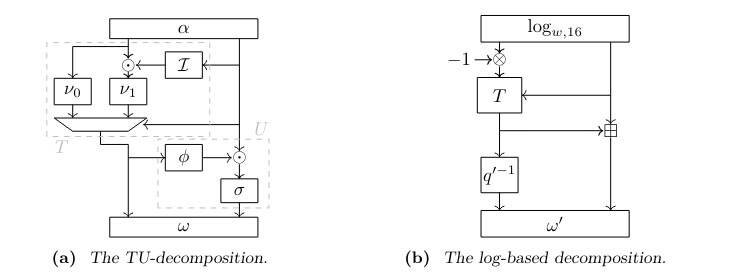
\includegraphics[scale=0.9]{contents/pics/decomposite.png}
        \caption{Разложение \(\pi\) в литературе}
        \label{fig:fig01}
\end{figure}

\subsubsection{TU-разложение}
Поскольку метод проектирования \(\pi\) не был опубликован, Бирюков и др. пытались найти дополнительные критерии проектирования или даже скрытую структуру, используя (и улучшая) техники из \cite{BP15}. Их результаты представлены в \cite{BPU16a, BPU16b}. Они показали, что \(\pi\) имеет TU-резложение, т.е. она аффинно-эквивалентна перестановке \((x, y) \mapsto (T_y(x), U_{T_y(x)}(y))\), где \(T_y\) и \(U_x\) являются 4-битными перестановками для всех \((x, y) \in (\mathbb{F}_2^4)^2\). Далее они представили разложение \(T\) и \(U\), как общую структуру \(\pi\), которая описана на Рисунке \ref{fig:fig01}a, где \(\nu_0\), \(\nu_1\) и \(\sigma\) являются 4-битными перестановками, \(\varphi\) является 4-битной функцией, такой, что \(\varphi(x) \neq 0\), а \(\mathcal{I}\) — мультипликативная инверсия в \(\text{GF}(2^4)\). Мультиплексор выбирает выход \(\nu_0\), если правая ветвь равна 0, и выход \(\nu_1\) в противном случае. Последними компонентами являются \(\alpha\) и \(\omega\), две 8-битные линейные перестановки, которые связаны следующим соотношением:

\begin{equation}
\{\alpha^{-1}(x||0), x \in \mathbb{F}_2^4\} = \{\omega(0||x), x \in \mathbb{F}_2^4\}.
\label{eq:01}
\end{equation}

Бирюков и др. начали с представления \(\pi\) с 8-битным линейным слоем \(L^*\), применяемым как ко входу, так и к выходу. То, что одна и та же функция применяется в обоих случаях, является следствием соотношения в Уравнении \ref{eq:01}. Они восстановили \(L^*\), используя визуальные шаблоны (паттерны) в LAT \(\pi\).

Еще одно свойство было отмечено в \cite{PU16}: \(\nu_0\) аффинно-эквивалентен дискретному логарифму в \(\text{GF}(2^4)\).

\subsection{Дискретный логарифм}

При исследовании S-блока белорусского стандарта блочного шифра BelT \cite{Bel11}, Перрин и Удовенко нашли совершенно другое разложение \(\pi\) \cite{PU16}. Действительно, они показали, что она имеет структуру, представленную на рисунке \ref{fig:fig01}b, т.е. она является композицией:

\begin{itemize}
    \item ''псевдологарифма'', т.е. перестановки, полученной путем инверсии ''псевдоэкспоненты'', которая построена как последовательность \([\alpha^0, \alpha^1, \alpha^2, \ldots, \alpha^{j-1}, 0, \alpha^j, \ldots, \alpha^{2^n-2}]\) для некоторого порождающего элемента \(\alpha \in \text{GF}(2^8)^*\);
    \item слоя операций модульной арифметики, которые они не смогли упростить;
    \item 4-битной перестановки \(q'^{-1}\);
    \item 8-битной линейной перестановки \(\omega'\).
\end{itemize}

Это разложение использует примитивный многочлен \(p_{\text{min}}(X) = X^8 \oplus X^4 \oplus X^3 \oplus X^2 \oplus 1\), который является порождающим многочленом конечного поля. Это первый примитивный многочлен степени 8, записанный в лексикографическом порядке, как видно, например, в Таблице C из \cite{LN97}. Он также является многочленом, который используется при построении конечного поля размера \(2^8\) в SAGE по умолчанию \cite{Dev17}.

\subsubsection{Связь между разложениями}

Эти разложения функционально эквивалентны, поскольку они соответствуют одной и той же перестановке \(\pi\), и, тем не менее, они имеют мало общего. При оценке TU-разложения, входная последовательность сначала проходит через линейный слой, отображающий \(\mathbb{F}_2^8\) в \((\text{GF}(2^4))^2\), а затем через \((a, b) \mapsto (a/b, b)\), за исключением случая, когда \(b = 0\). С другой стороны, для оценки логарифмического разложения сначала нужно использовать вариант дискретного логарифма. Какова связь между этими операциями?

Поэтому кажется удивительным существование обоих разложений. Более того, ни одна из них не кажется естественным выбором для построения S-блока. Эти наблюдения привели Перрина и Удовенко к следующему выводу \cite{PU16}: ''Мы считаем более вероятным, что [TU-разложение и логарифмическое разложение] являются следствием сильной алгебраической структуры, которая использовалась для проектирования [\(\pi\)], возможно, связанной с экспонентой в конечном поле. Тем не менее, ''мастер-разложение'', из которого вытекали бы другие, остается невыясненным. К сожалению, пока российские спецслужбы не обнародуют свою стратегию разработки, их точный процесс, скорее всего, останется загадкой, хотя бы потому, что существуют альтернативные варианты разложения: какой из них существует по замыслу, а какой является лишь побочным эффектом этого замысла?''

В следующем разделе будет рассмотрено то, что, по нашему мнению, является этим ''мастер-разложением''. Оно опирается на дискретный логарифм, который связывает его со вторым разложением, и оказывается, что TU-разложение, идентичное тому, что было в [BPU16a], всегда возможно для перестановок с подобной структурой. В данной работе утверждается, что это новое разложение, вероятно, и есть то, которое было задумано разработчиками.